% Datei: chapters/05_atommodelle/01_thomson_rosinenkuchenmodell.tex

\subsection{Thomsons Rosinenkuchenmodell: Elektronen als eingebettete Teilchen}
\index{Thomsons Atommodell}
\index{Rosinenkuchenmodell}
\index{Elektron}
\index{Atommodell}

Nach der Entdeckung des Elektrons war klar, dass das Atom keine unteilbare
Kugel sein konnte. Es musste eine innere Struktur besitzen. Das Elektron war
ein Bestandteil des Atoms, aber damit stellte sich sofort eine neue Frage:
Wie sind diese negativ geladenen Teilchen im Atom angeordnet?

J. J. Thomson entwickelte dazu ein frühes Atommodell. In diesem Modell besteht
das Atom aus einer positiv geladenen Grundmasse, in die die negativ geladenen
Elektronen eingebettet sind. Da das Atom nach außen elektrisch neutral ist,
muss die positive Ladung die negative Ladung der Elektronen insgesamt
ausgleichen.

Anschaulich wurde dieses Modell später als Rosinenkuchenmodell bezeichnet.
Die Elektronen entsprechen dabei den Rosinen, die in einer positiv geladenen
Masse verteilt sind. Der Begriff ist bildhaft, aber er beschreibt die zentrale
Idee recht gut: Die Elektronen sind nicht frei außerhalb des Atoms angeordnet,
sondern befinden sich innerhalb einer ausgedehnten positiven Ladungsverteilung.
\FloatBarrier
\begin{figure}[H]
	\centering
	 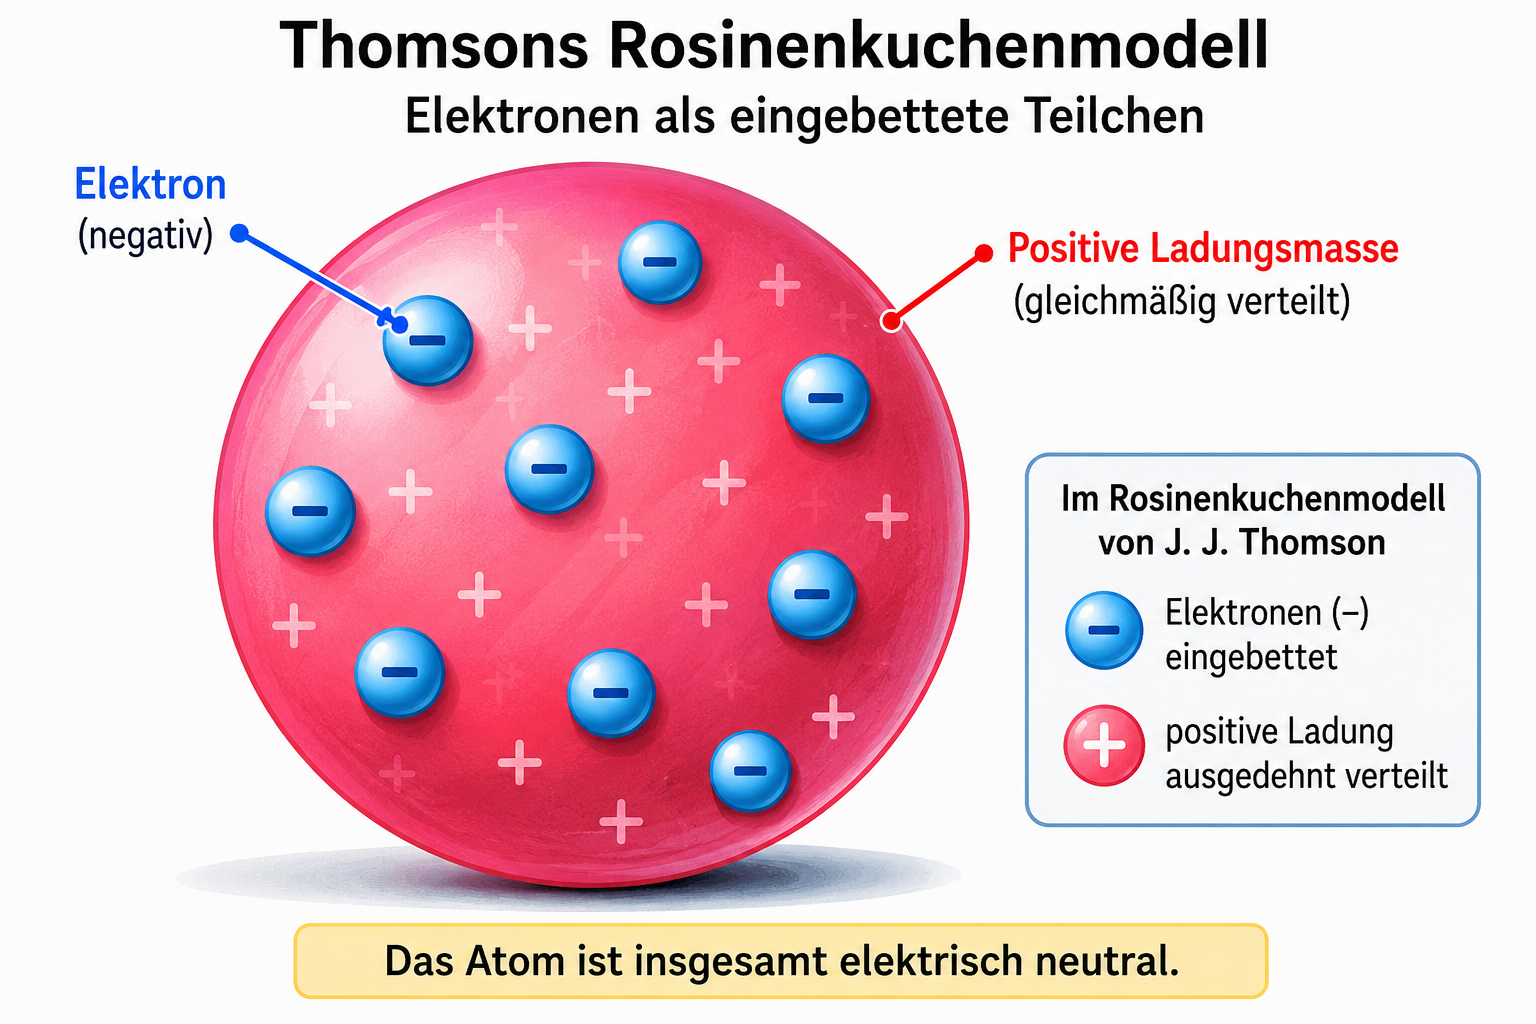
\includegraphics[width=0.65\textwidth]{bilder/rosinenkuchenmodell}
	\caption{Schematische Darstellung des thomsonschen Atommodells. Die negativ
		geladenen Elektronen sind in eine positiv geladene Grundmasse eingebettet.}
	\label{fig:thomson_rosinenkuchenmodell}
\end{figure}

Das Modell war ein wichtiger Schritt, weil es das Elektron erstmals als
Bestandteil des Atoms einordnete. Gleichzeitig blieb es noch stark klassisch
gedacht. Es gab keinen Atomkern, keine Elektronenschalen und keine Vorstellung
von quantisierten Energiezuständen.

Aus heutiger Sicht ist das Rosinenkuchenmodell falsch. Sein Wert liegt aber
darin, dass es eine erste konkrete Antwort auf die neue Situation nach der
Entdeckung des Elektrons gab. Das Atom war nicht mehr unteilbar. Es war ein
zusammengesetztes System aus positiver und negativer Ladung.

Die entscheidende Schwäche des Modells zeigte sich wenige Jahre später durch
das Goldfolienexperiment von Rutherford. Dort wurde sichtbar, dass die positive
Ladung nicht gleichmäßig im Atom verteilt ist, sondern in einem winzigen,
massereichen Atomkern konzentriert sein muss. Damit wurde Thomsons Modell
abgelöst.

\begin{HistoryBox}[Thomsons Rosinenkuchenmodell]
	
	\label{box:thomson-rosinenkuchenmodell}
	Das thomsonsche Atommodell war der erste Versuch, das neu entdeckte Elektron
	als Bestandteil des Atoms zu verstehen. Die negativ geladenen Elektronen sind
	in eine ausgedehnte positive Ladungsmasse eingebettet.
	
	Das Modell erklärt die elektrische Neutralität des Atoms, kennt aber noch
	keinen Atomkern. Genau daran scheiterte es später beim Goldfolienexperiment
	von Rutherford.
	
\end{HistoryBox}